% !TeX root = ../main.tex

\chapter{Introduction}
The \IIC{} is a serial communication protocol used to attach lower-speed peripheral ICs to processors and micro-controllers in short-distance and intra-board communication. As reported in Randall Hyde's book \cite{hyde2022book}, before \IIC{} bus, different components of a computer system communicated with one another using 8 to 32 data lines and some number of address signals, requiring more space and increasing the amount of noise to deal with. In 1982 \cite{wu2022basic}, Philips Semiconductors (now NXP Semiconductors) developed the \IIC{} protocol, alleviating these problems using just 2 wires: the data line (SDA) and the clock line (SCL).

\section{Circuit description}

The system is composed of one or more masters, that can write or read, and several slaves, all connected to the bus, with a bidirectional communication. Typical implementation is shown in Figure \ref{fig:i2c_implementation}:

\begin{figure}[htbp]
    \centering

    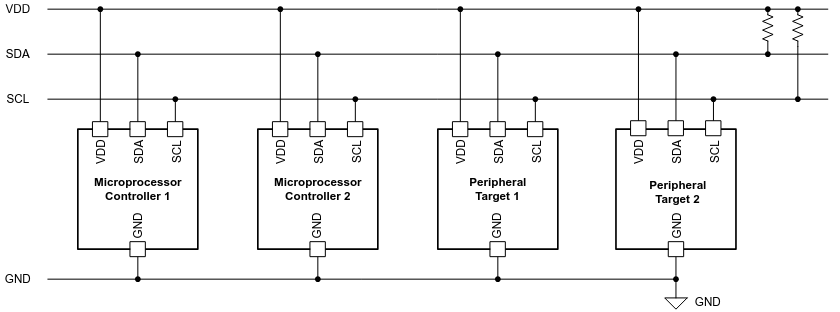
\includegraphics[width=0.8\textwidth]{../imgs/i2c_implementation.png}
    
    \caption{\IIC{} implementation \cite{wu2022basic}.}
    \label{fig:i2c_implementation}
\end{figure}

\section{Possible applications}
The \IIC{} protocol is widely adopted in embedded systems, thanks to the low power consumption and space optimization, to interface microcontrollers with various peripheral ICs, such as sensors, execution elements and human interaction devices. One example is presented in \cite{pintilie2019i2c}, where the protocol is used to connect a master, the embedded computer, to all the devices installed for a smart home. 

\section{Writing Master}

One possible implementation is the one reported in this documentation: the Writing Master. The device acts as the master in the \IIC{} protocol, but can only write data; no reading operation is implemented. The design is shown in Figure \ref{fig:i2c_wm_design}:

\begin{figure}[htbp]
    \centering
    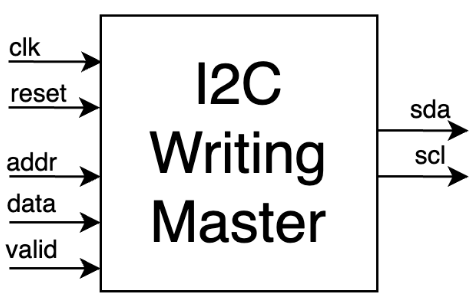
\includegraphics[width=0.5\textwidth]{../imgs/i2c_wm_design.png}
    
    \caption{Writing Master design}
    \label{fig:i2c_wm_design}
\end{figure}

All the signals in input to the Writing Master come from a processor or a microcontroller to indicate when to communicate, using the \texttt{valid} signal, to whom, using the \texttt{addr} signal, and what, using the \texttt{data} signal. After receiving the essential information, the master starts to communicate with the slave indicated in the \texttt{addr} signal using the \texttt{scl} and \texttt{sda} signals. The \texttt{sda} signal is used by the slave too during the acknowledgment phase. The clock used to communicate with the slave is 32 times slower than the system clock (\texttt{clk} signal). A possible use case of this implementation is with actuators or display drivers, for example, where the master sends a command and they simply answer with the ACK signal.
